\documentclass[letterpaper]{article}

\usepackage[utf8]{inputenc}
\usepackage[sort, colon]{natbib}
\usepackage{alifexi}
\usepackage{color}
\usepackage{amsmath}
\usepackage{amssymb}
\usepackage{commath}

\usepackage[colorlinks=true,citecolor=blue,linkcolor=blue]{hyperref}
\usepackage{flushend}

\newcommand\todo[1]{\textcolor{red}{TODO: #1}}

\newcommand{\E}{\mathbb E}

\title{Human-level control through deep reinforcement learning}
\author{C\'{e}dric Simar, Antoine Passemiers, Stanislas Gueniffey \and Robin Petit \\
\mbox{}\\
Universit\'{e} Libre de Bruxelles \\
\{Cedric.Simar, apassemi, sgueniff, robpetit\}@ulb.ac.be}

\begin{document}
\maketitle

\begin{abstract}

  Reinforcement learning is a subarea of machine learning inspired by neuroscience, where learners have to select actions with
  regards to the environment state and receive a reward accordingly. Each agent's objective is to maximize its cumulative reward across its whole lifetime,
  subdivided into episodes. In the traditional framework of reinforcement learning and more specifically in Q-learning,
  researchers usually deal with a small discrete space to represent the values of Q. This is no longer sufficient if one desires to describe the environment state
  as an image of raw pixels. In consequence, we introduce deep Q-learning methods, which have been found to be really effective in mapping raw pixels
  to abstract high-level features. In deep Q-learning, the estimation of Q-values for a given action are produced using deep neural networks,
  which consist of many neural layers stacked on top of each other.
  These techniques have revealed themselves to be able to beat human experts at playing Atari games
  by learning only from visual features. Despite the current progress, learning how to take complex decisions on the basis of high-dimensional visual data remains an
  ongoing challenge. In particular, because of the instability of neural networks, we also explored state-of-the-art dueling architectures to enhance performance
  by separating the high-level representation of states and action values (rewards).

\end{abstract}

\section{Introduction}

We designed the agent in such a way that it selects actions according to its beliefs about future rewards, and its only objective is to maximize its total
cumulative reward. More formally, this cumulative calculation starts from present time $t$ and is computed as follows:
\begin{equation}
  Q^{*}(s, a) = \max_{\pi} \E\left[ \sum_{k \geq 0}r_{t+k}\gamma^k \; \big| \; s_t = s, a_t = a; \pi\right].
\end{equation}
where $\pi = P(a | s)$ is a behavior policy, $t$ is the current step, $r_t$ is the reward for step $t$, $a_t$ is the action selected at time $t$,
and $\gamma$ is the discount factor. Thus, we can describe the Q-value as the present value of all future rewards at current step $t$,
with respect to the environment state and the action selected at $t$.

Because of the very high dimensionality of input visual features, it is not reasonable to consider using a table for storing all Q-values.
Instead, one can design a learnable function that maps pixel values to a single row of this table, thus a vector of Q-values whose length is the size
of the action space. For that purpose we used a Deep Q-Network (DQN) to approximate this function, as in the original DQN article~\citep{mnih2015human}, since feedforward Neural Networks
are known to be universal function approximators (Theorem 2 in~\cite{hornik1991approximation}).
A DQN is a particular instance of Convolutional Neural Networks (CNN) and is composed of a stack of neural layers~\citep{lecun1998gradient}. One characteristic of CNNs is the
presence of convolutional filters that maps pixel luminance to more abstract features. Each filter (or kernel) is locally connected to its output, which
allows the convolutional layer to capture the local information of the pixels, contrary to what dense (fully-connected) layers do. This procedure is greatly
inspired by the notion of receptive field introduced by Hubel and Wiesel~\citep{Hubel1962}.
Let $Q(s, a; \theta_i)$ be the Q-value approximation function represented by the neural network, parameterized by its weights $\theta$ at time step $i$.

The huge breakout effect of the DQN was that it has shown to be a first step towards general artificial intelligence~\citep{togelius2015ai}, meaning an
algorithm that is not only good at learning one particular task but several of them. Even though the DQN needs to be trained for about a million steps
on each Atari game, it gets good at most of them and better than human at 22 of the 49 experimented~\citep{mnih2015human}.

Since we are handling visual features, we used screen frames as environment state representations. Each frame is a (210 x 160) color image sampled at
a frequency of 60 Hz. We denote the environment state at current step $t$ by $s_t$. The agent gathers experience by incorporating new experience samples
to its history. An experience is a tuple $e_t = (s_t, a_t, r_t, s_{t+1})$ appended to the experience history immediately after being generated.
To prevent the agent from forgetting the history and increase the bias towards most recent experience samples, we have recourse to the experience
replay algorithm ~\citep{adam2012experience}. One can straightforwardly implement it as a uniform sampling algorithm that returns random experience samples at each step.
We compared this technique to a more efficient approach called prioritized experience replay~\citep{DBLP:journals/corr/SchaulQAS15}.
To emphasize the importance of the memory replay mechanism, we compared the results obtained using prioritized experience replay, regular
experience replay, and no experience replay.

Every 4 steps of the Q-learning, the agent builds a minibatch from its memory (either one of the three mechanisms we just mentioned):
this minibatch is used by the DQN to process one step of stochastic gradient descent. In this way the values of Q are estimated iteratively and
refined over time. The deep neural network incorporates minimal prior knowledge about the environment: the only assumption lies in the number of
outputs in the last hidden layer, which has been set as the number of actions. In every Atari game, the action space is discrete, finite and constant over time:
this allows us to determine the output shape of the neural network depending on the game itself. The number of actions made available by the environment
cannot be inferred by the DQN during training phase.

Also we compared DQN, as well as other state-of-the-art deep reinforcement learning architectures, to simpler reinforcement learning techniques (including
random action selection) using a normalized performance metric. The latter is formalized as below:
\begin{equation}
    P = 100 \times (\text{score} - RAS) / (HS - RAS),
\end{equation}
where P designates the normalized performance, RAS the random action selection score, and HS the human score obtained in average by our
Space Invaders professional gamer \textbf{Stanislas Gueniffey}. By normalizing in this manner, the random action selection score RAS results in
a normalized performance of 0\% and the human score results in a normalized performance of 100\%.

Finally it has been pointed out by the original DQN conceptors that DQN has an ability to learn by acquiring experience generated from policies
other than its own. \todo{On peut en faire qqch pas vrai ?}

\section{Methods}

Our source code is available at \url{https://github.com/RobinPetit/Learning-Chaos}.

We developed our models with the support of the Arcade Learning Environment~\citep{bellemare13arcade}. This gives the opportunity to either
retrieve the environment state as a raw image (for deep reinforcement learning research) or as a state of the RAM (for classic reinforcement learning
applications). Because of the very high dimensionality of raw images, we applied some preprocessing steps on them. These steps are also aimed at
removing some artifacts produced by the Atari architecture. More specifically, the flickering effect implies that some game sprites only appear
in one out of two frames. An easy solution consists in taking the pixelwise maximum value between the current frame and the previous frame.
Then the sample size has been reduced by a factor of three by mapping RGB values to the pixel luminance, using the following formula:
\begin{equation}
    \text{Luminance} = 0.299 \times R + 0.587 \times G + 0.114 \times B.
\end{equation}

After mapping the three color channels to a unique channel, the number of pixels has also been reduced. Each input image as been rescaled to a
$84 \times 84$ pixel grid.

The perceived rewards of the agent have all been reduced to be either $-1$ for a negative reward, $0$ for a session with no reward, and $+1$
for a positive reward, i.e. at any time $t$: $r_t \in \{-1, 0, +1\}$. No intermediate or larger reward is available to the learning algorithm.
This allows to learn without any previous knowledge on the particular game the DQN is trained on. Yet some rewards can be highly different (in Pac-Man likes,
eating a cherry gives 100 points, a banana gives 5000, and eating a ghost gives $2^n \times 100$ with $n$ the number of eaten ghosts in a single run).
This could be improved by adaptive normalization~\citep{van2016learning}.

As estimating the whole $Q^*$ function is practically not performable, $Q^*$ is estimated by a non-linear function depending on $\theta$ such that:
\begin{equation}
	\forall s \in S : \forall a \in A(s) : Q(s, a; \theta) \simeq Q^*(s, a).
\end{equation}

In this situation, the non-linear function is the neural network, and $\theta$ represents its weights.

The interest of using a neural network is to be able to update the weights such that at each time step $t$, the weights are $\theta_t$, and:
\begin{equation}
	\forall s \in S : \forall a \in A(s) : Q(s, a; \theta_t) \xrightarrow[t \to +\infty]{} Q^*(s, a).
\end{equation}

Therefore, the NN is trained by minimizing the Huber loss~\citep{huber1964robust} with $\delta=1$ of the Bellman equation (by a -- stochastic -- gradient descent).
The Huber loss $H_\delta$, parameterized by $\delta \in {\mathbb R^*}^+$, is a continuous function (also $C^1$ but not $C^2$) defined by the mean
squared error on a small neighbourhood of $0$, and by the absolute value outside this neighbourhood:
\begin{equation}
	H_\delta : \mathbb R \to \mathbb R : x \mapsto \begin{cases}\frac 12x^2                                &\text{ if } \abs x \leq \delta,\\
	                                                            \delta\left(\abs x - \frac 12\delta\right) &\text{ otherwise.}\end{cases}
\end{equation}

The interest of the Hubert loss is to bound the gradient of the loss between $-1$ and $+1$, and has (\todo {probably}) been shown to increase
stability.~\todo{check if this has a proper reference or drop it}

\subsection{Neural Network architecture}

The Deep Q-Network is a Convolutional Neural Network (CNN) composed of three convolutional layers followed by a fully-connected layer, 
leading to the final output fully-connected layer.
Between each of these units a non-linear function is applied, which result in Rectifier Linear Units (ReLU) \citep{krizhevsky2012imagenet}, but Exponential Linear Units (ELU) could
also be used since it has been shown to be more performant in classification and decision tasks~\citep{DBLP:journals/corr/ClevertUH15}, but also
Flexible Rectified Linear Units~\citep{qiu2017flexible}.

The first convolutional layer outputs 32 $20 \times 20$ images from a $84 \times 84$ image, using $8 \times 8$ filters and a stride of $4$. The second one outputs
64 images of size $9 \times 9$ from the previous 32, using filters of size $4 \times 4$ and a stride of $2$; and the third and last convolutional layer
applies 64 filters of size $3 \times 3$ with stride $1$ on the 64 subimages of the previous layer to output $7 \times 7$ images.

These are then reshaped into a column vector (of size $7 \times 7 \times 64 = 3136$) and fed into the first fully-connected layer with 512 neurons,
which is then connected to the last layer (again fully-connected) which corresponds to the output with the same size as the action space (6 in the
case of Space Invaders).

We also reimplemented a Dueling Deep Q-Network (DDQN) in which the high-level representation of states and action values are separated.
For this purpose,the same convolutional architecture as before was kept, but the output of the last convolutionel layer was split in two streams of
equal sizes (each stream input size is the same as the output size of the last convolutional layer), then the resulting tensors have been flattened.
The first stream, which is designed to represent the potential advantage per action, is fully-connected to 6 neurons (one per action), while the second stream
contains a dense representation of the state value and is fully-connected to a single neuron.

The last layer of the DDQN outputs Q-value estimates by evaluating the following formula:
\begin{multline}
    Q(s, a; \theta, \alpha, \beta) = V(s; \theta, \beta) + \\ ( A(s, a; \theta, \alpha) - \frac{1}{|\mathcal{A}|} \Sigma_{a'} A(s, a'; \theta, \alpha) )
\end{multline}
where $V$ is the output of the state-value stream, $A$ is the output of the advantage-per-action stream, $s$ is the input state (image), 
$\alpha$ are the parameters of the state-value stream's fully-connected layer, $\beta$ are the parameters of the state-value stream's
fully-connected layer, $\theta$ are the parameters of the rest of the network, and $\mathcal{A}$ is the discrete action space.

\subsubsection{Implementation}
The neural networks have been implemented using the software library Tensorflow \citep{tensorflow2015-whitepaper}.
Thus our models consist of data flow graphs designed in a symbolic programming fashion, where each node of a graph is an operation
and each edge is a data tensor.

\subsection{Weight update}

In order to reduce oscillation in $Q$ estimations, two separate neural networks have been used: the first one, denoted $Q$ and called the \textit{action-value}
network is the one used in action prediction, and the second one denotes $\hat Q$ and called the \textit{target action-value} network is used when
updating the weights. This particular method holds for both DQN and DDQN The parameters of $Q$ are denoted by $\theta$ as previously, and the parameters of $\hat Q$ are denoted by $\theta^-$.

Every 4 steps, at time $t$, a minibatch of 32 past experiences $\left\{(s_{t_j}, a_{t_j}, r_{t_j}, s_{t_j+1})\right\}_{j=1}^{32}$ is selected uniformly from the
memory in order to perform a Stochastic Gradient Descent (SGD), thus the average of the gradients of the loss function on each experience is used to update
the weights. As mentioned above, the loss function is a Huber loss function and is defined as:
\begin{equation}
	H_1\left(y_j - Q(s_{t_j}, a_{t_j}; \theta)\right),
\end{equation}
with $y_j$ set either to $r_j$ if $s_{t_j}$ is a final state (i.e. either the loss of a game or a forced end of episode) or to
$r_j + \gamma\max_{a' \in A(s_{t_j})}\hat Q(s_{j+1}, a'; \theta^-)$ otherwise; therefore using the target action-value network.

The $\hat Q$ target action-value network is then copied back from the action value network $Q$ every 10,000 steps.

\section{Results}

\begin{figure*}
  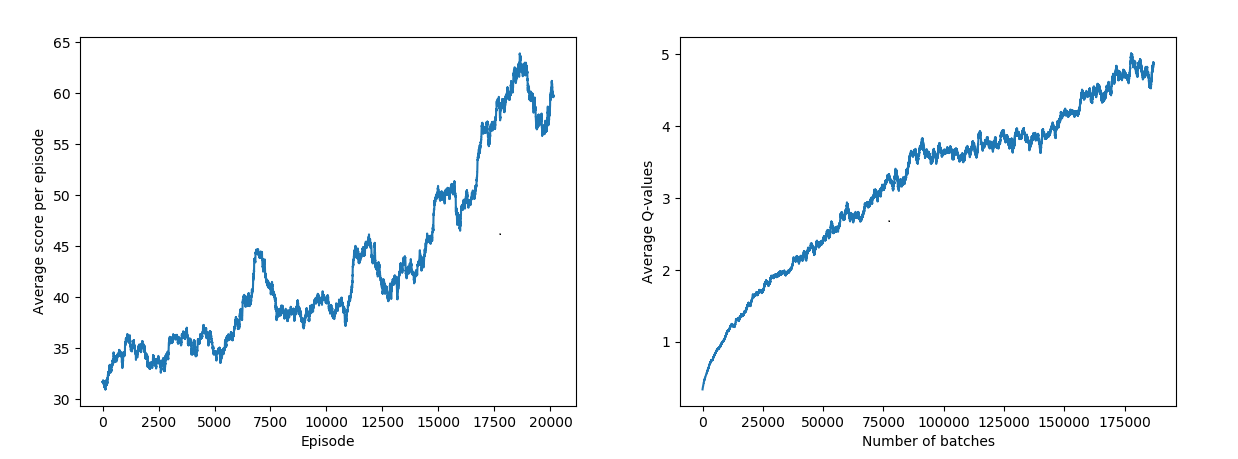
\includegraphics[width=\textwidth]{figures/dqn_uniform}
  \caption{(Left) Total score per episode during a learning phase of 1.000.000 steps, smoothed using a moving average with a window of size 2000.
     (Right) Estimation of Q, averaged across actions, for each batch during a learning phase of 1.000.000 steps and smoothed using a moving average
      with a window of size 2000.}
\end{figure*}

Figure~\ref{fig:t-SNE}\todo{Link the right figure} shows a 2-dimensional representation of the last fully connected hidden layer, i.e. a 512-dimensional
vector. The method of \textit{projection} that was used is t-SNE~\citep{maaten2008visualizing}, which is part of the manifold learning algorithms, also
called \textit{Nonlinear Dimensionality Reduction}~\citep{lee2007nonlinear}.

The implementation of t-SNE that was used is the one from Scikit-Learn~\citep{scikit-learn}, the Python library.

  \todo{Magnifique plot T-SNE avec des couleurs et des gifs et des trucs qui font beep et qui font boop}~\citep{wattenberg2016how}

\section{Discussion}

  \todo{Amélioration: Double dueling DQN}~\citep{DBLP:journals/corr/WangFL15}

\section{Acknowledgements}

  \todo{Remercier Lenaerts, Nowe, Google, OpenAI, Markov}

\newpage
\footnotesize
\bibliographystyle{apalike}
\bibliography{article}

\end{document}
